\documentclass[10pt,a4paper, openany]{book}
\usepackage[utf8]{inputenc}
\usepackage[english]{babel}
\usepackage{amsmath}
\usepackage{amsfonts}
\usepackage{amssymb}
\usepackage{graphicx}
\usepackage{color}
\usepackage{xcolor}
\usepackage{lmodern}
\usepackage{tablefootnote}
\usepackage[sc]{mathpazo}
\usepackage{booktabs}
\usepackage{hyperref}
\usepackage{fancyhdr}
\usepackage{multirow}
\hypersetup{pdftex, colorlinks=true,linkcolor=black}

\newcommand\mytokens[1]{\mytokenshelp#1 \relax\relax}
\def\mytokenshelp#1 #2\relax{\allowbreak\grayspace\tokenscolor{#1}\ifx\relax#2\else
 \mytokenshelp#2\relax\fi}
\newcommand\tokenscolor[1]{\colorbox{gray!20}{\textcolor{black}{%
  \ttfamily\mystrut\smash{\detokenize{#1}}}}}
\def\mystrut{\rule[\dimexpr-\dp\strutbox+\fboxsep]{0pt}{%
 \dimexpr\normalbaselineskip-2\fboxsep}}
\def\grayspace{\hspace{0pt minus \fboxsep}}

\usepackage{floatrow}
\newfloatcommand{capbtabbox}{table}[][\FBwidth]
\usepackage{blindtext}

\author{Armando Brandonisio}
\title{\textbf{Software chapter}\\COMPASS thesis}

\begin{document}
\maketitle
\tableofcontents \newpage

\chapter{Software development}
SiPMs spectrum is theoretically composed by gaussian peaks that follow Poisson distribution as discussed in Cap (..).\\
In this chapter I show basics for a simple Monte Carlo model and its application for SiPM spectrum simulation. Furthermore I created an analysis software that simplifies and automatizes physical results extracted by SiPMs spectra. I wrote all scripts and code using Python language. 

\section{Monte Carlo simulation}
Monte Carlo method solves a problem by generating suitable random numbers and observing that fraction of the numbers obeying some property or properties. The method is useful for obtaining numerical solutions to problems which are too complicated to solve analytically. In physics-related problems, Monte Carlo methods are quite useful for simulating systems with many coupled degrees of freedom, such as fluids, disordered materials, strongly coupled solids, and cellular structures.\\
In my work I used Monte Carlo method to simulate a SiPM output spectra in the ideal case: no \emph{cross-talk} and no \emph{afterpulses}. The expected spectrum is a gaussians sequence  which centroids correspond to each photo-electron value. This result would be a convergence test for fitting processes and physical properties interpretation.\\
First I simulated a uniform distribution and than a gaussian spectrum to emulate a detected X-Ray photo-peak.\\
I performed all analysis data and simulation using \verb|Python v.3.5.2| and the following libraries:
\begin{itemize}
\item \verb|Numpy v.1.10.4|
\item \verb|Numba v.0.23.1|
\item \verb|LmFit v.0.93|
\item \verb|Pandas v.0.18.1|
\item \verb|Scipy v.0.17.0|
\item \verb|Matplotlib v.1.5.1|
\item \verb|accelerate_cudalib v.2.0|
\item \verb|Stoner v.0.5|

\end{itemize}

\subsection{Discrete uniform distribution}
The discrete uniform distribution has \emph{pdf} 
\begin{equation}
f(x;a,b) =  \frac{1}{b-a+1}, \quad x \in \{ a, ..., b\}
\end{equation}
where $a,b \in \mathbb{Z}, b\geq a$ are parameters. The discrete uniform distribution is used as a model for choosing a random element from $\{a,...,b\}$ such that each element is equally likely to be drawn.\\
There is a easy way to compute a uniform distribution using \verb|Python| language: \verb|Numpy| random libraries. A dedicated routine to compute uniform distributions is \verb|numpy.random.uniform|\footnote{np.random.uniform:\url{http://docs.scipy.org/doc/numpy/reference/generated/numpy.random.uniform.html}}.\\
Generate random numbers could be a hard work for CPU computers, than I setted \emph{bins} and \emph{events} such that total time computation was $\sim 2 s$\footnote{Tested with Intel Core i7-5500U (Broadwell) 2.4 GHz up to 3.0 GHz}. I chose 500 bins with $10^5$ events. I tested the same program with \verb|accelerate_cudalib| library too that compute code with Nvidia GPU cores (CUDA). The same result was achieved in $\sim 0.1 s$\footnote{Tested with Nvidia 920M and CUDA toolkit 7.5}. This could be a start point for more realistic simulations.\\
I interpreted bins as collected charge in a range of 0-40 $e^-$, and rate as counts per second (normed to 0.5). The result in Fig~\ref{fig:1}.

\begin{figure}[!h]
\begin{center}
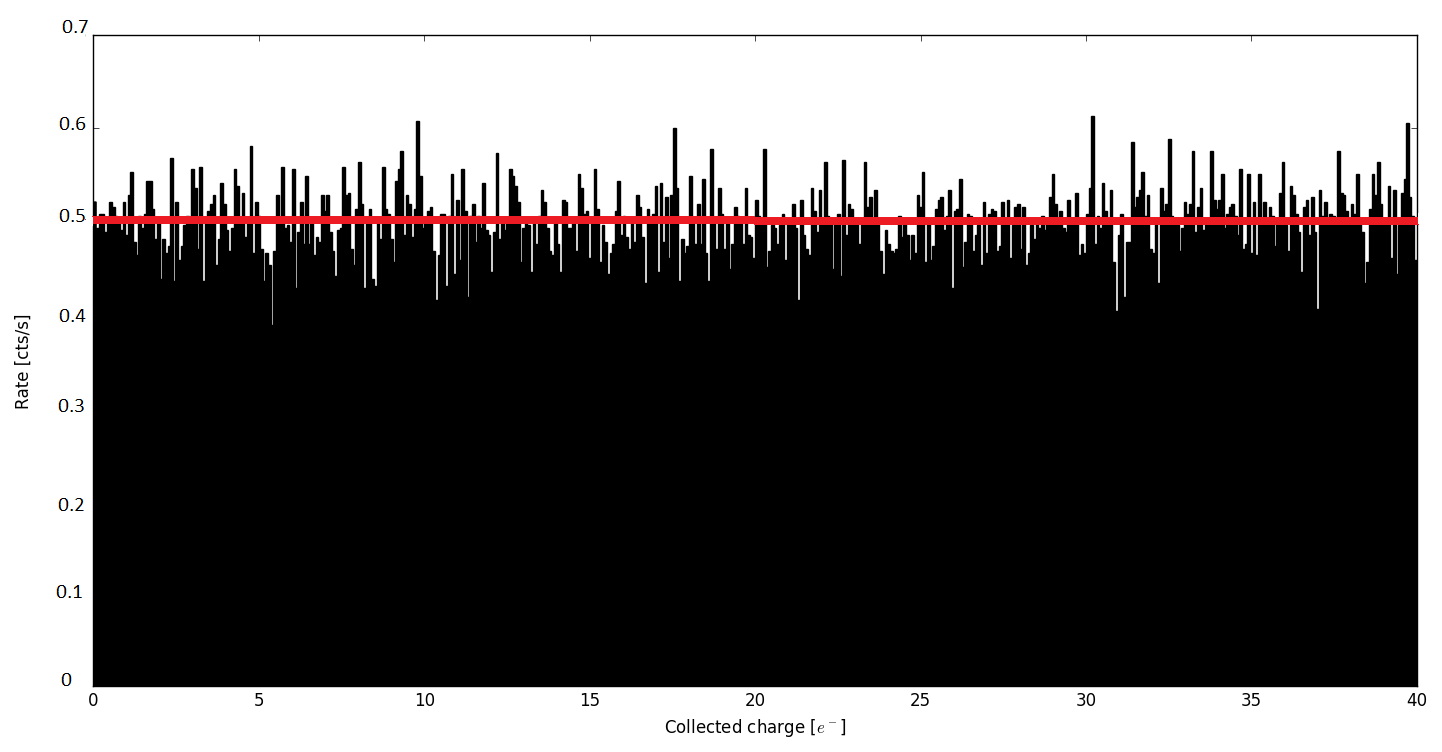
\includegraphics[scale=0.32]{imm/sim_const_un.png}
\end{center}
\caption{Discrete uniform distribution}
\label{fig:1}
\end{figure}
Simulated spectra have a density bin of $\sim 12.5\; bins/e^-$. The real spectrum acquired with LCT5/1 (+3V), Ortec474 (gain:4x2, int: 50$\mu s$) and MCA dynamic range of 0-5V divided in 4096 channels, has a density bin of $\sim 40\; bins/e^-$, where bins are MCA channels.\\
To generate gaussian spectra I used \verb|numpy.random.normal| \footnote{numpy.random.normal \url{http://docs.scipy.org/doc/numpy/reference/generated/numpy.random.normal.html}} routine. As discussed in Chapter (..)   SiPM spectra follow Poissonian distribution, and then gaussian curves for each photo-electron value (N-PE) depends on $\sigma_i\sqrt{N}$:
%\begin{equation}
%\sigma_{i+1} = \sigma_i \sqrt{i+1}
%\end{equation}
An example of gaussians sequence is reported in Fig~\ref{fig:2}. I used \verb|numpy.concatenate|\footnote{numpy.concatenate \url{http://docs.scipy.org/doc/numpy/reference/generated/numpy.concatenate.html}} routine to sum events of different distributions on the same bin, in order to get the correct analytical convolution. 

\begin{figure}[!h]
\begin{center}
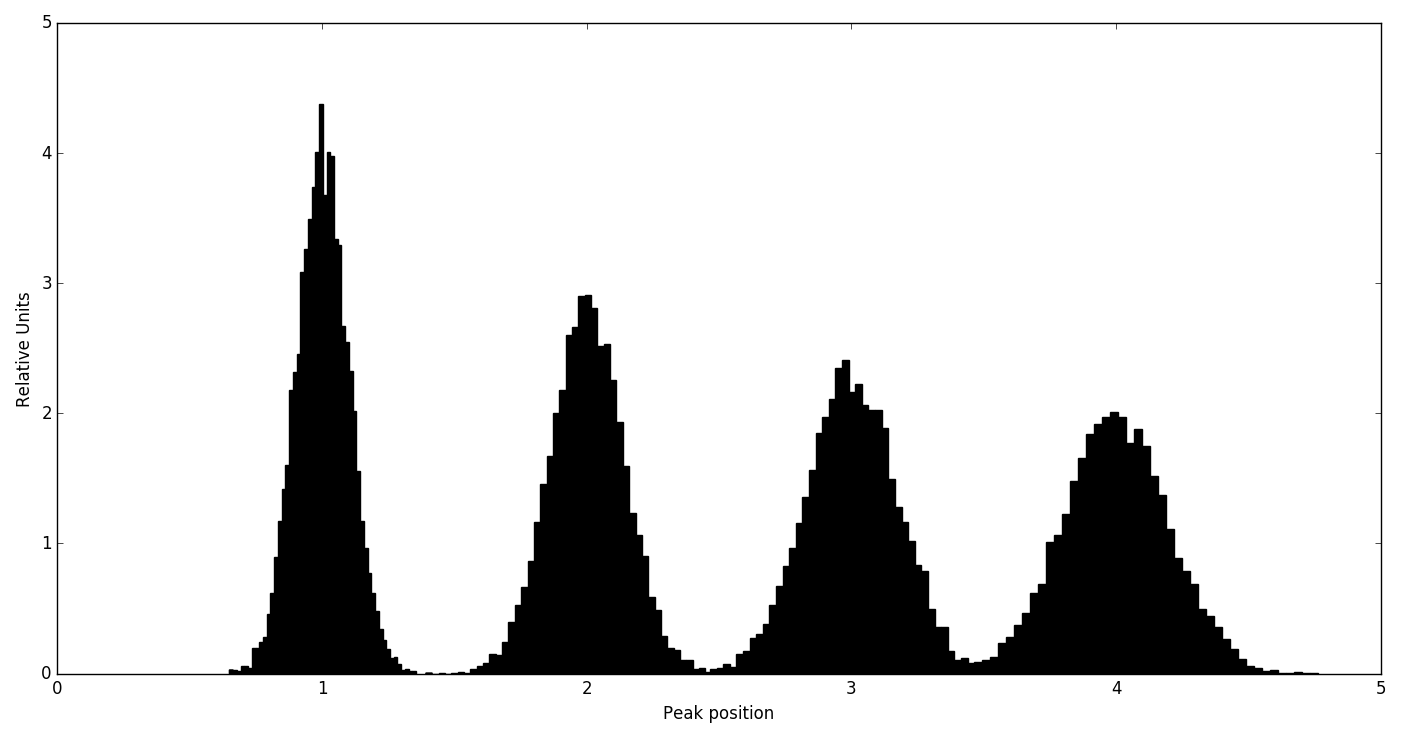
\includegraphics[scale=0.28]{imm/peaks.png}
\end{center}
\caption{Convolved gaussian distributions.}
\label{fig:2}
\end{figure}
I replicated uniform distribution showed in fig~\ref{fig:1} with SiPM-like distribution, and the results is plotted in fig~\ref{fig:3}. The resolution for each PE is $\sim 10\%$.
\begin{figure}[!h]
\begin{center}
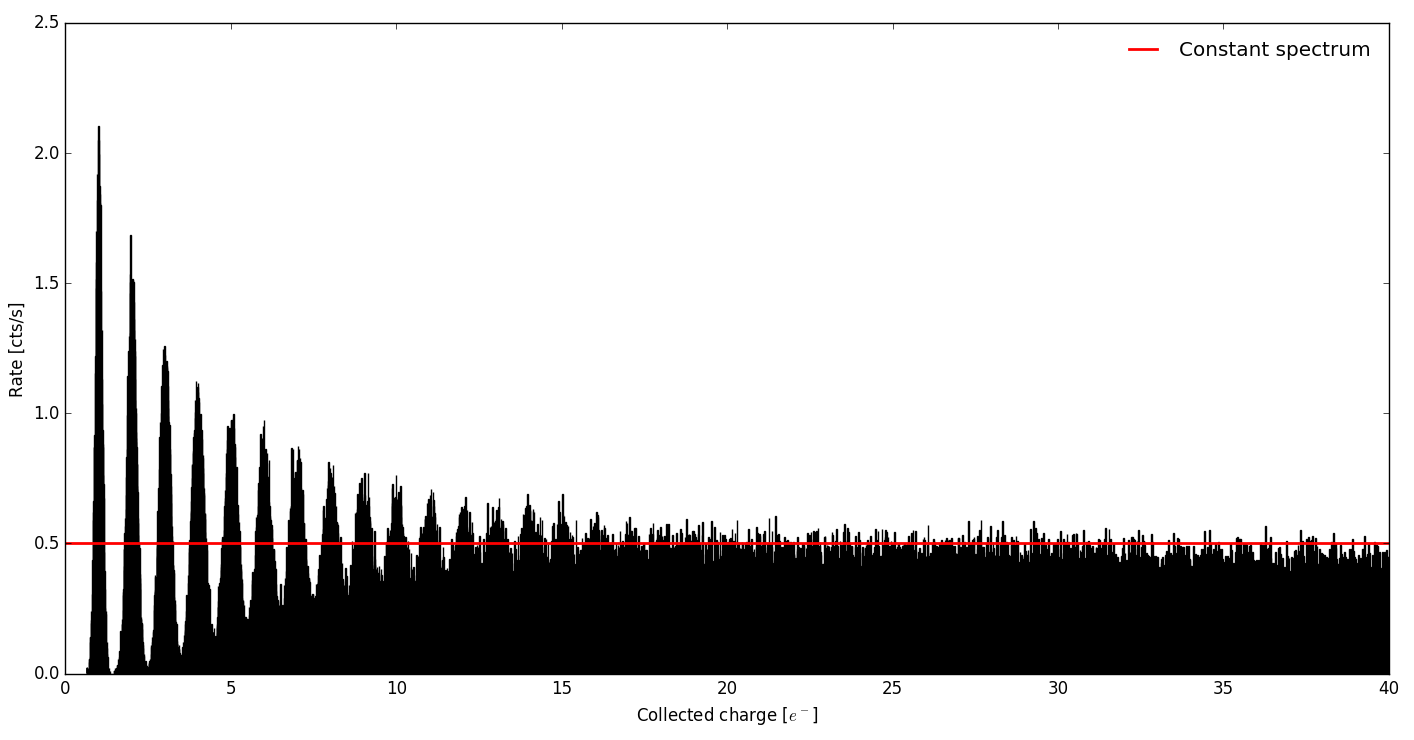
\includegraphics[scale=0.3]{imm/sim_const2.png}
\end{center}
\caption{Discrete uniform distribution simulated with SiPM criterion.}
\label{fig:3}
\end{figure}

First N-Pe values are well resolved from each other (quantized spectrum), but for $N>10$ the convolution effect makes single N-PE peak unresolved and for this the spectrum becomes discrete uniform distribution with the same value of fig~\ref{fig:1} (0.5 cts/s).

\subsection{Gaussian distribution}
The normal or standard Gaussian distribution has pdf:
\begin{equation}
f(x; \mu , \sigma^2) = \frac{1}{\sigma \sqrt{2\pi}} e^{-\frac{1}{2}\frac{(x- \mu)^2}{\sigma^2}} = N(\mu, \sigma)
\end{equation}
or for a non-normed distribution:
\begin{equation}
f(x; \mu , \sigma^2, A) = A e^{-\frac{(x- \mu)^2}{\sigma^2}} = G(\mu, \sigma, A)
\end{equation}
The aim of this section is to explain how I simulated a gaussian distribution seen from a SiPM.\\
First I created a normed gaussian centered in $14e^-$ and $\sim 78\%$ of resolution as laboratory measurements reported in Chap(Instrumental), that I called $N_T$. (fig~\ref{fig:4}).
\begin{figure}[!h]
\begin{center}
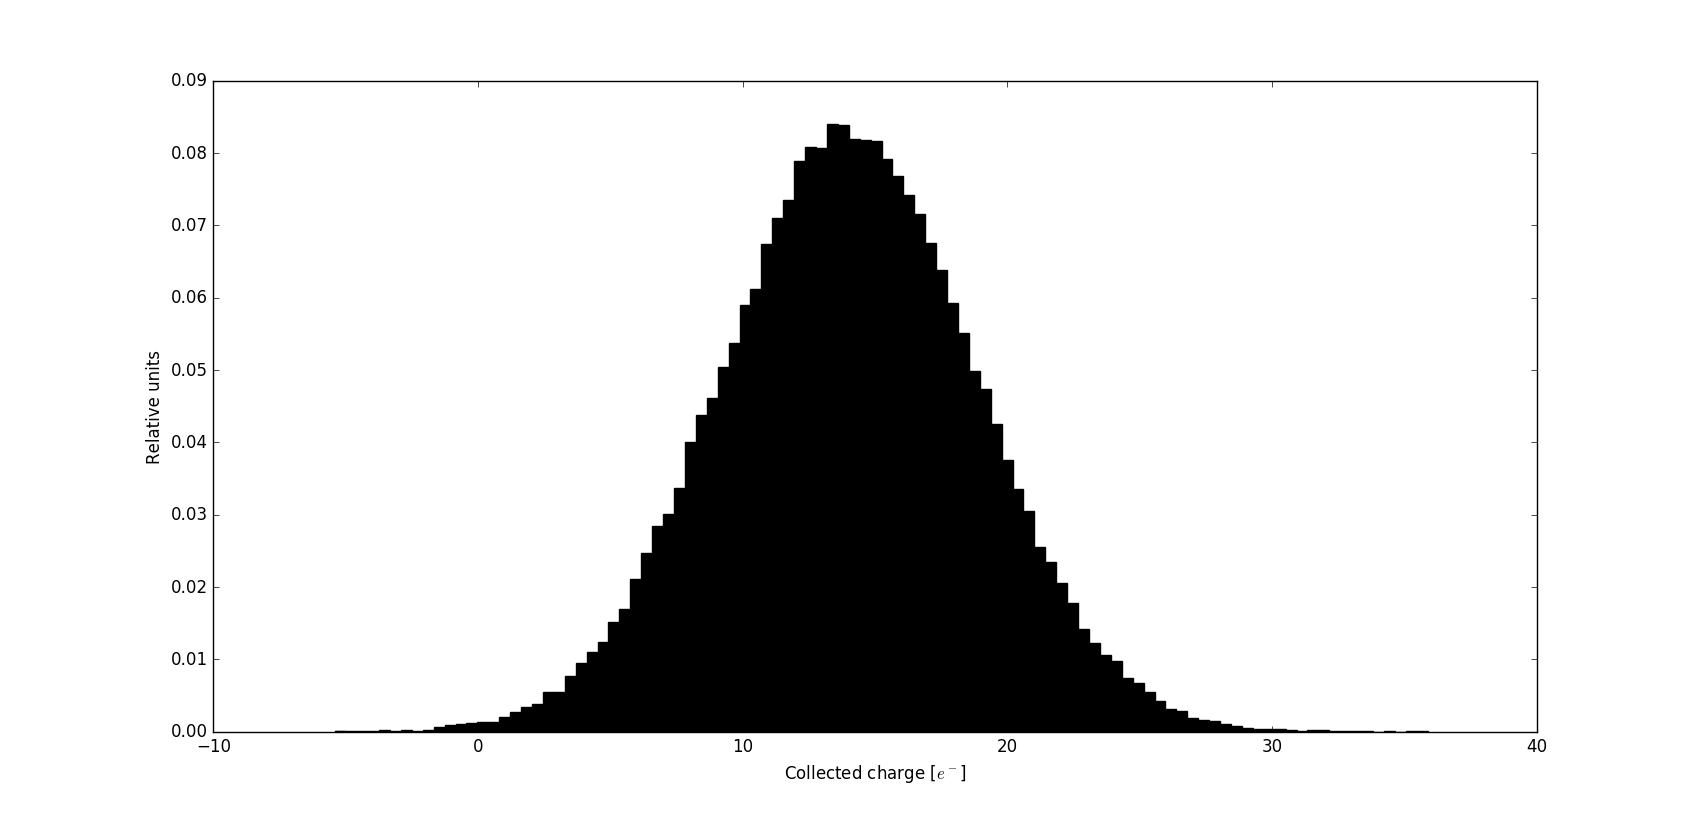
\includegraphics[scale=0.3]{imm/gaussian.png}
\end{center}
\caption{Gaussian normed distribution $N_T$.}
\label{fig:4}
\end{figure}

I calculated each SiPM n-PE distribution ($G_N$ as follows:
\begin{equation}
G_n = N(n,\sigma\sqrt{n}) \cdot N_T(x=n)
\end{equation}
where $N(n,\sigma\sqrt{N}$ is a normed gaussian centered in $n$ and with required $\sigma$ variation, and $N_T(x=n)$ is the starting distribution computed in $x=n$. The result of this step is showed in fig~\ref{fig:5}.\\
\begin{figure}[!h]
\begin{center}
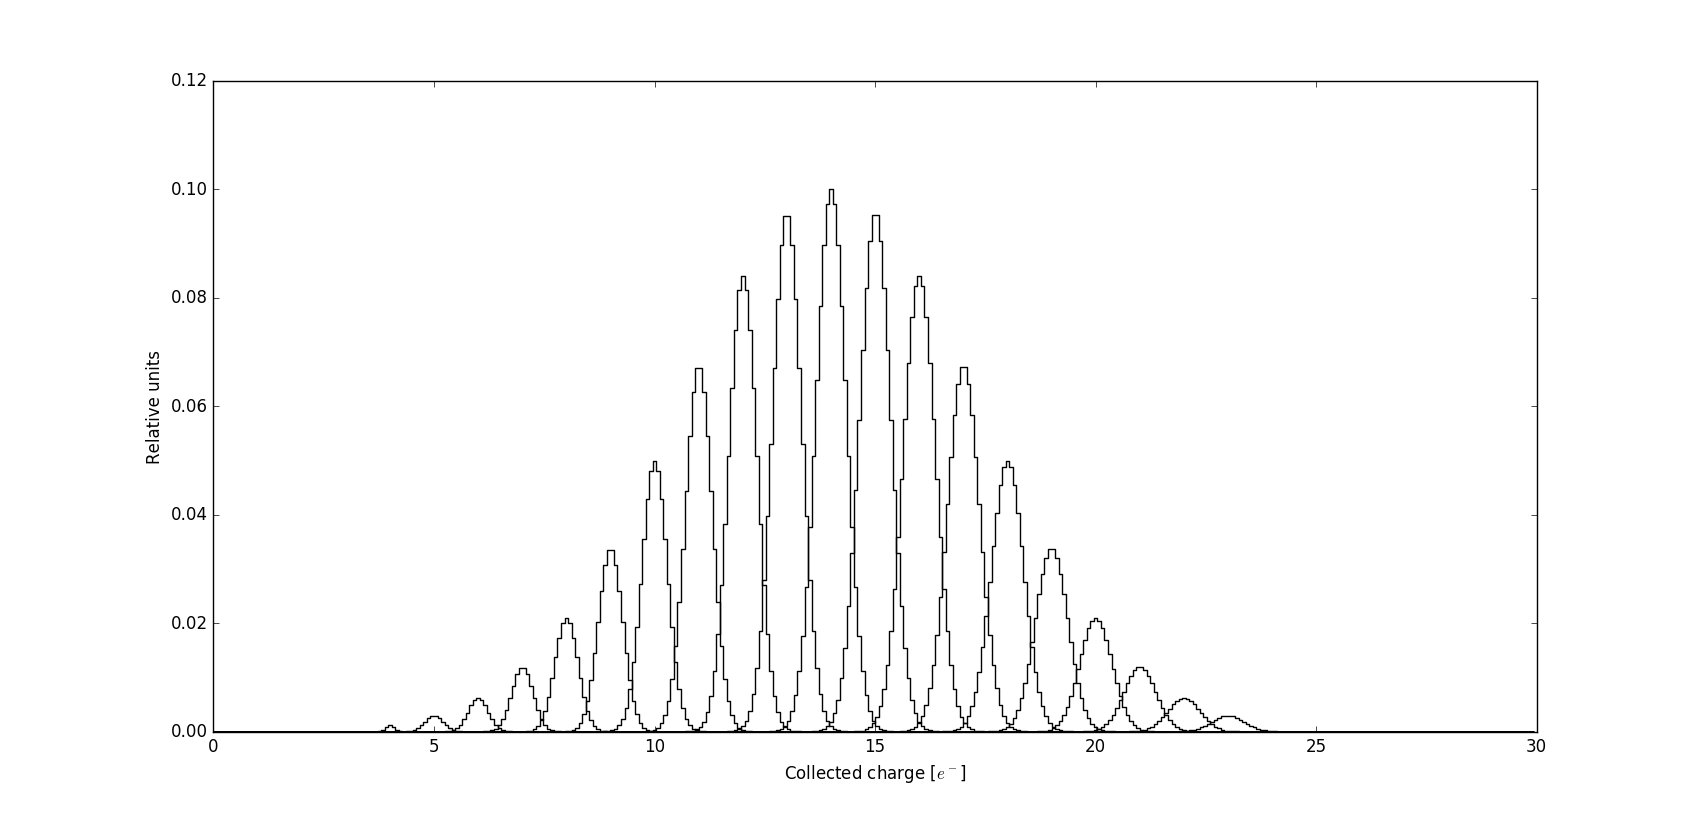
\includegraphics[scale=0.3]{imm/gauss2.png}
\end{center}
\caption{n-PE distribution for a gaussian function.}
\label{fig:5}
\end{figure}
\newpage
The equivalent gaussian distribution for a SiPM is calculated by:
\begin{equation}
G_{tot} = \sum_n N(n,\sigma\sqrt{n}) \cdot N_T(x=n)
\end{equation}
and showed in fig~\ref{fig:6}.
\begin{figure}[!h]
\begin{center}
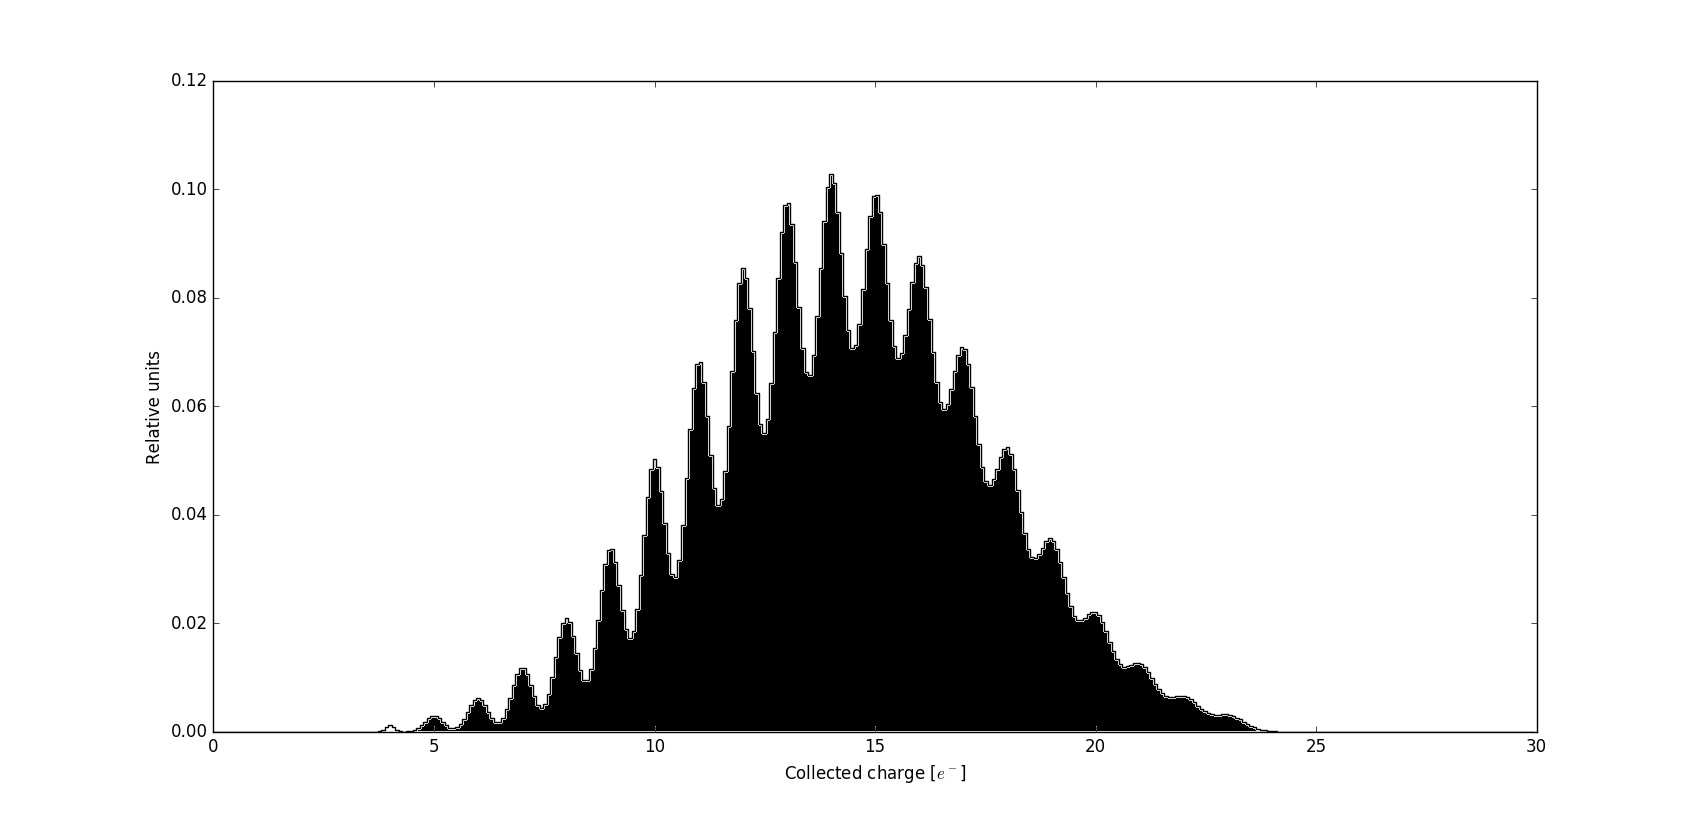
\includegraphics[scale=0.3]{imm/gauss3.png}
\end{center}
\caption{n-PE distribution for a gaussian function.}
\label{fig:6}
\end{figure}

\section{Fit strategy}
After simulating ideal SiPM spectra, the fundamental step is to study a fit strategy that converges to original spectra calculated in fig.~\ref{fig:1} and fig.~\ref{fig:4}.\\
Basically we have a mixture of gaussians to fit. Fitting process is not stable when there are a lot of functions due to large number of degrees of freedom. For this is fundamental to fix some parameters or choose initial values. In my work I found very useful to choose gaussian peaks as fit initial values, because are intrinsic properties of n-PE distribution and are well distinguished form each other until are resolved. This process is explained in Par~\ref{par:peak}. Than I performed a multi-gaussian fit (Par~\ref{par:mg}) from which I obtained information on single n-PE FWHM (par.~\ref{par:fwhm}), area of each one and their linearity in position calibrated in charge (par.~\ref{par:lin}).\\
This process makes possible to extract physical spectrum (or information) from SiPM characteristic output signal. From this one starts the last algorithm that extrapolate information about resolution, total area and collected charge of a X-ray photo-peak (par.~\ref{par:area}).
The whole logical process is schematized and showed in Fig~\ref{fig:7}

\begin{figure}[!h]
\begin{center}
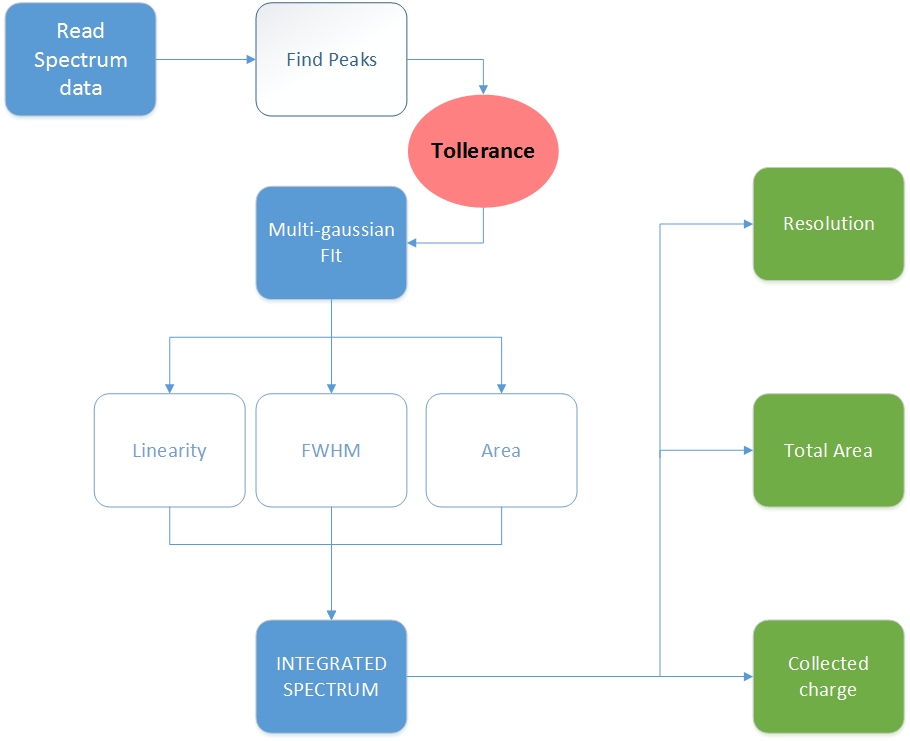
\includegraphics[scale=0.45]{imm/schema.png}
\end{center}
\caption{Software logical scheme.}
\label{fig:7}
\end{figure}

\subsection{Peak-finder}
\label{par:peak}
Peak finding is a tricky and often required task in experimental data analysis. When a functional form is known, it is possible to fit the data to this functional form. However, often a more numerical approach is required. The \verb|AnalyseFile.peaks()|\footnote{\url{http://pythonhosted.org/Stoner/classesStoner.Analysis.AnalyseFile.peaks.html}} provides a relatively simple and effective method for doing this.\\
The algorithm used is to differentiate the data with a Savitsky-Golay filter\footnote{\url{https://en.wikipedia.org/wiki/Savitzky-Golay_filter}}, which in effect fits a polynomial locally over the data. Zero crossing values in the derivative are located and then the second derivative is found for these points and are used to identify peaks and troughs in the data.\\
In this package there is a \verb|significance| parameter too.
The \verb|significance| parameter controls which peaks and troughs are returned. If \verb|significance| is a float, then only peaks and troughs whose second derivatives are larger than \verb|significance| are returned. If \verb|significance| is an integer, then maximum second derivative in the data is divided by the supplied \verb|significance| and used as the threshold on which peaks and troughs to return. The \verb|width| and \verb|poly| keywords are used to control the order of polynomial and the width of the window used for calculating the derivative. A lower order of polynomial and wider width will make the algorithm less sensitive to narrow peaks.\\
I integrated \verb|AnalyseFile.peaks()| in my own algorithm that i called  \mytokens{find_peak}. This script is equipped of an optimized version of \verb|significance| parameter that I named \verb|tollerace|. This function allows to improve robustness of peak-search for a multi-gaussian spectrum avoiding probability of revealing statistical fluctuations as peaks and it is based on \emph{peak-to-valley} ratio.\\ An example of script core is reported as follows:
\begin{quote}
\begin{verbatim}
d, x, y = Data                         #Acquisition data
error = sqrt(rate)                     #Counts error
a = #peak-to-valley ratio in %

for i in range(1, n+1)
    min(n) = min(y[n+1] - y[n])
    max(n) = max(y[n+1] - y[n])
    tollerance = min(n)/max(n)

def find_peak(n, rate, peaks)
    if tollerance > a
       d.peaks(width=8,poly=4,significance=tollerance)
       returns peaks
    else peaks == nan
         quit = True
d.find_peak()	
\end{verbatim}
\end{quote}

While \verb|tollerance| is less then a certain value, the script detects all peaks over the threshold, otherwise it stops to find other peaks. In fig~\ref{fig:8} is reported a comparison between high and low \verb|tollerance| value.

\begin{figure}[!h]
\begin{center}
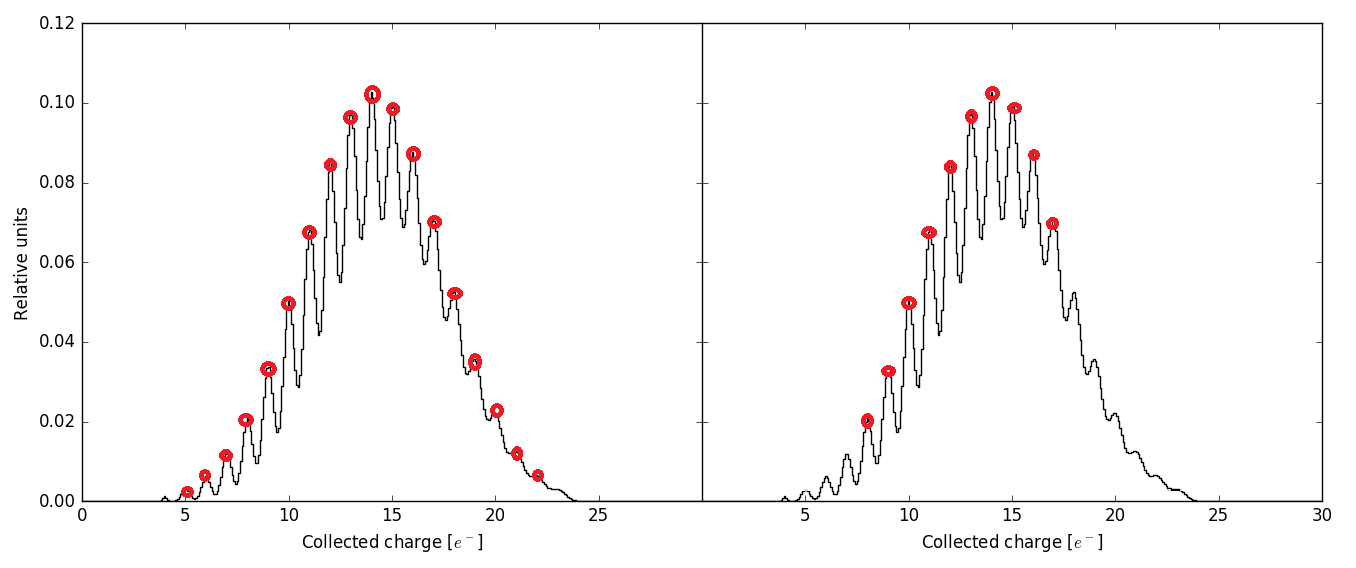
\includegraphics[scale=0.4]{imm/gp2.png}
\end{center}
\caption{\emph{Left:} 5\% tollerance value. \emph{Right:} 50\% tollerance value}
\label{fig:8}
\end{figure}
\newpage
\subsection{Multi-gaussian fit}
\label{par:mg}
Previous paragraph gives fit initial values to starting analysis. A Multi-gaussian fit, with more than 20 gaussians, is a really challenge test for  common fitting tools convergence. Peaks-positions values make fit works only if \verb|tollerance| value is appropriate. Choosing right \verb|tollerance| parameter is not a lucky process, but strongly depends on 'purity' and symmetry of spectrum. For SiPM ideal spectra tollerance($\tau$) is $\sim 5\%$ for a smoothly fit convergence. For LCT5/1 spectra @+3V $\tau \sim 30-35 \%$ due to small distortions (afterpulses, pile-up, etc.) and for really distorted signals like LCT4/10 $\tau > 65\%$. This could be a threshold for a not-analyzable SiPM spectra.\\
The fitting script, that I called \mytokens{mg_fit}, has a code core showed as follows:  
\begin{verbatim}
def mg_fit(x, *params):
    y = np.zeros_like(x)
    for i in range(0, len(params), 3):
        ctr = params[i]
        amp = params[peaks[i]]
        wid = params[i+2]
        y = y + amp * np.exp( -((x - ctr)/wid)**2)
    return y
\end{verbatim}

that is a simple iteration using \verb|lmfit| libraries for fitting models and statistical tools, and \mytokens{find_peak} results to force convergence. I analyzed constant and gaussian simulated spectra from previous paragraphs. Results in Fig.~\ref{fig:9} and Fig.~\ref{fig:10}.

\begin{figure}[!h]
\begin{center}
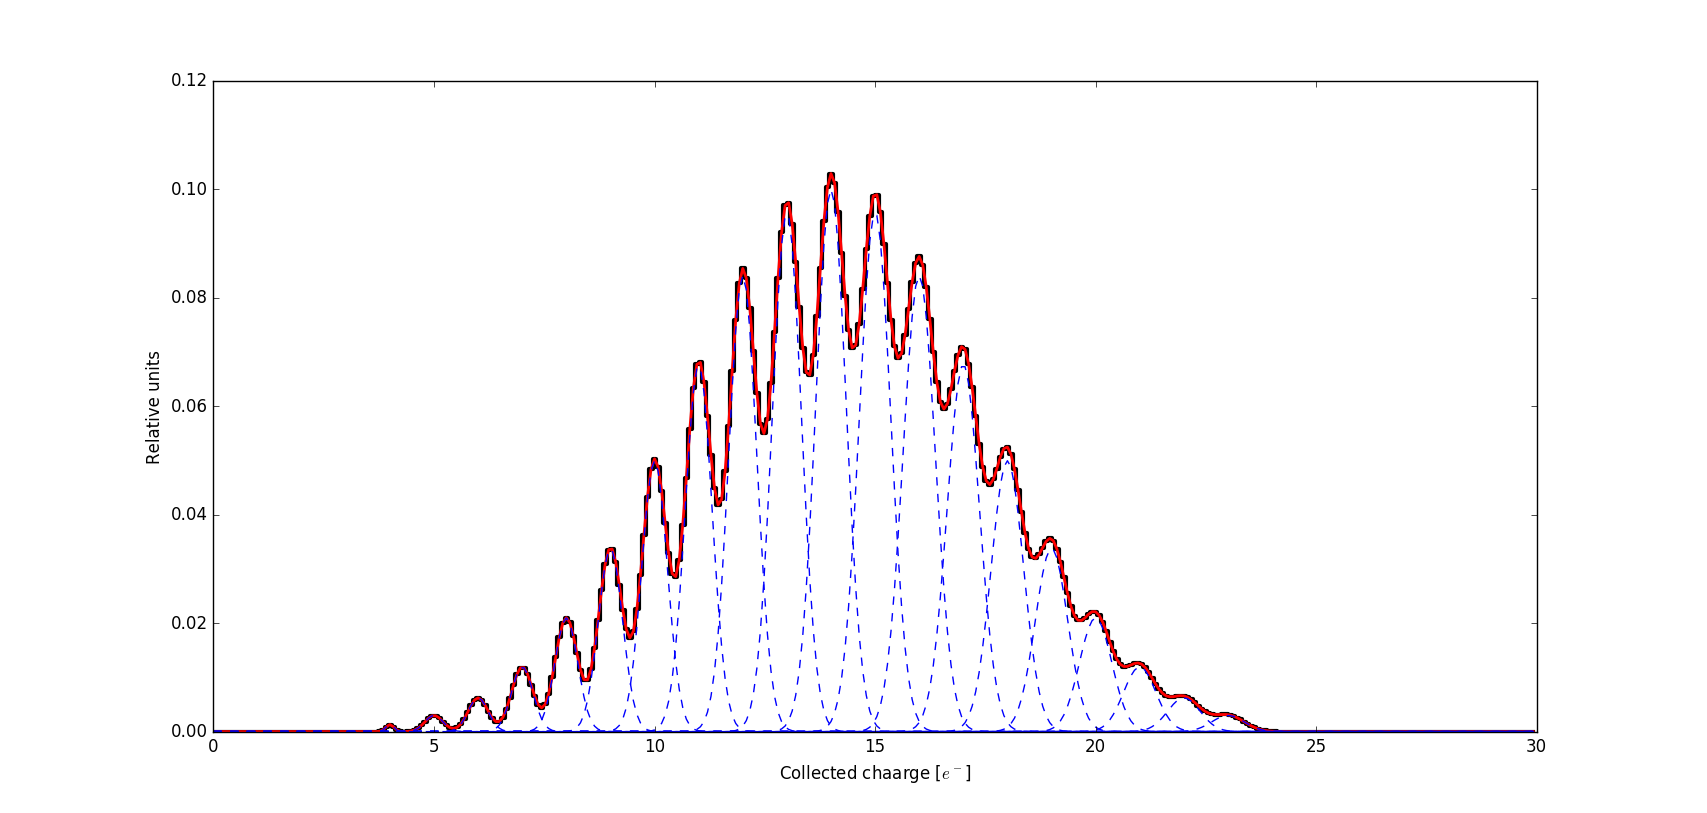
\includegraphics[scale=0.3]{imm/fit.png}
\end{center}
\caption{Fit of gaussian distribution spectrum}
\label{fig:9}
\end{figure}

\begin{figure}[!h]
\begin{center}
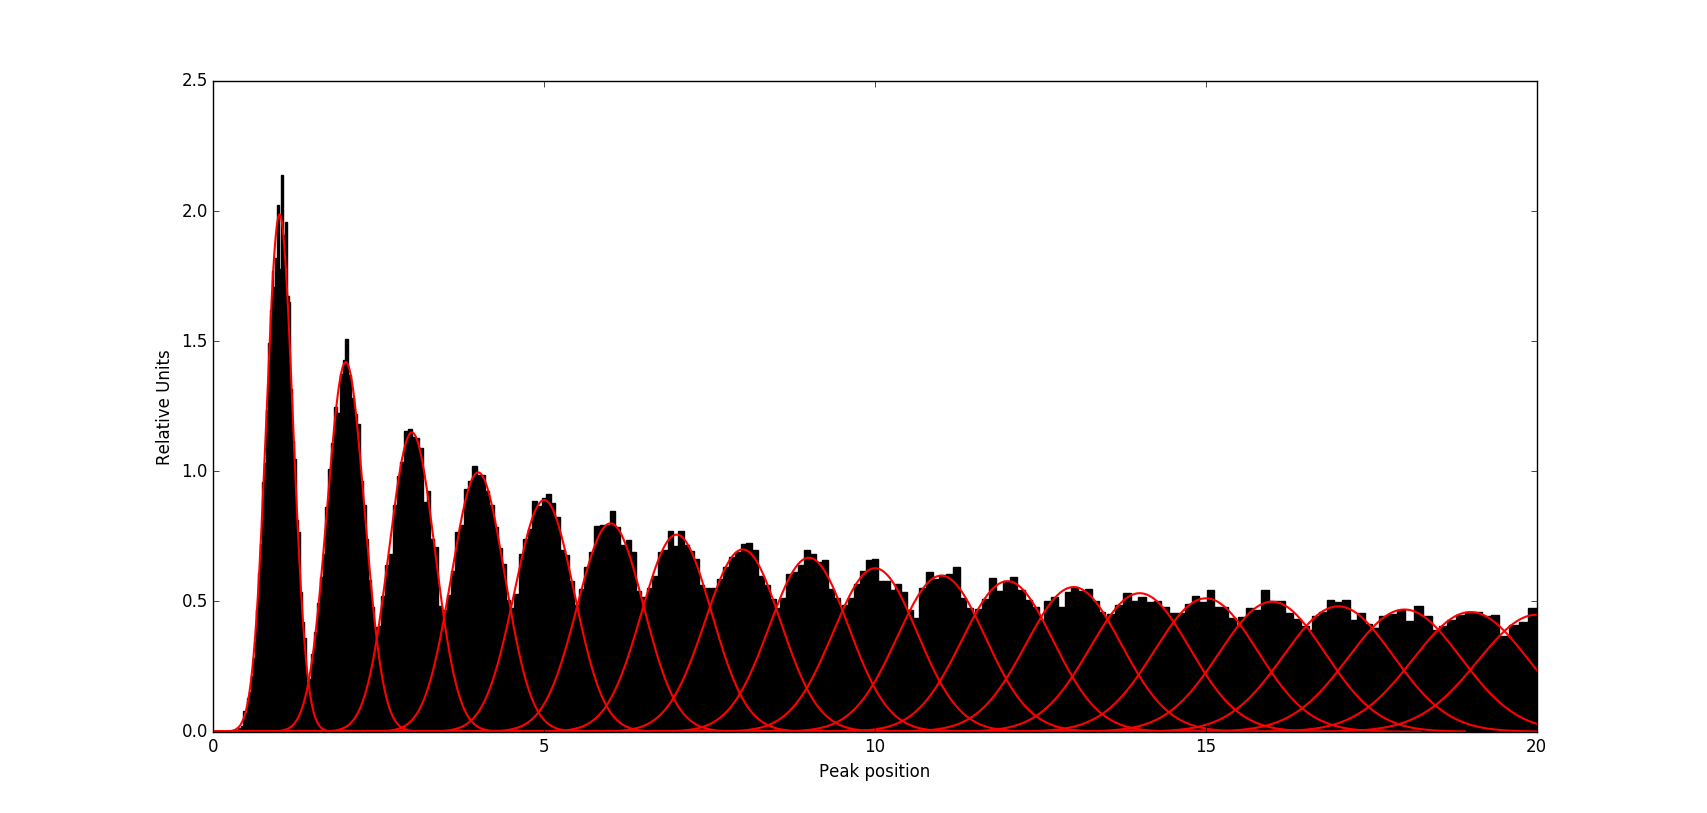
\includegraphics[scale=0.3]{imm/fit2.png}
\end{center}
\caption{Fit of constant distribution spectrum.}
\label{fig:10}
\end{figure}
\newpage
\subsection{Study of $FWHM/\sqrt{N}$ linearity}
\label{par:fwhm}
SiPM poissonian distribution is a predictable feature of detected spectra. One of the most important proof for poissonian distribution test is the $\sigma_{PE_n}/\sqrt{n}$ linearity, or the equivalent $FWHM_{PE_n}/\sqrt{n}$. When this fraction is not constant (on a certain uncertainty), the analyzed spectrum could be affected by noisy factors as electronic instability or pile-up. This feature is easy to detect because comes from \mytokens{mg_fit} results. I created a secondary script called \mytokens{fwhm_lin} that saves FWHM values in a independent array which divides it for $\sqrt{n}$. I tested this script on previous results. Gaussian and constant simulated spectra have the same statistical 'birth' than I can choice the first one as representative for both. \mytokens{fwhm_lin} results are showed in fig~\ref{fig:11}

\begin{figure}[!h]
\begin{center}
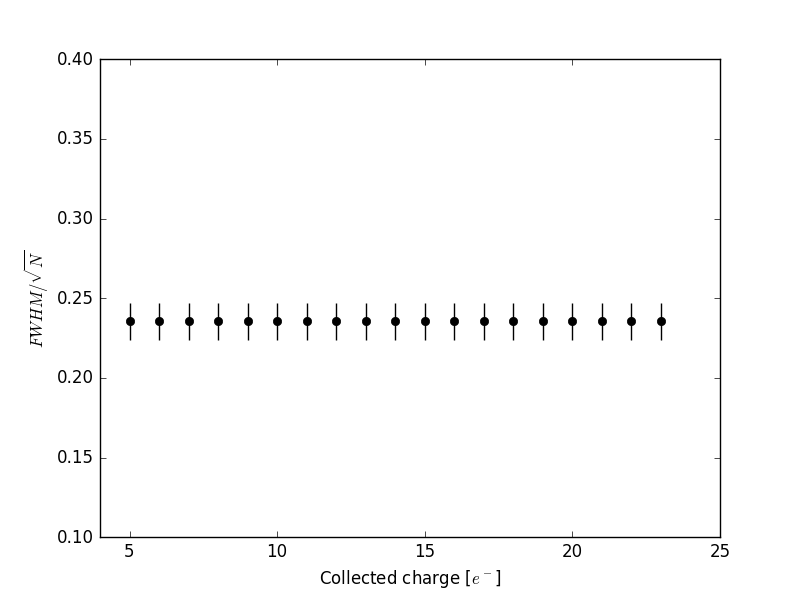
\includegraphics[scale=0.5]{imm/fwhm.png}
\end{center}
\caption{\mytokens{fwhm_lin} results for $FWHM/\sqrt{N}$ linearity.}
\label{fig:11}
\end{figure}

The results is obviously constant for an ideal spectrum and the value is $\sim 0.23$. This is a SiPM intrinsic number that is strictly linked to PE resolution since:
\begin{equation}
Res = \frac{FWHM}{n}
\end{equation} 
therefore
\begin{equation}
\frac{FWHM}{\sqrt{n}} = Res \cdot \sqrt{n}
\end{equation}
Thus ratio lower values are better for a good single PE resolution and for a higher resolved PE peaks.

\subsection{Linearity of $n$-PE position}
\label{par:lin}
Another fundamental SiPM feature is the n-PE position linearity. For a calibrated spectrum (in charge), difference from n-PE peaks should be $\sim 1e^-$. I created a simple script called \mytokens{position_diff} that saves n-PE centroid values from \mytokens{mg_fit} in a independent array and makes the following operation:
\begin{equation}
PE_{n+1} - PE_{n}
\end{equation}
Results from gaussian spectrum is showed in fig~\ref{fig:12}.\\
\begin{figure}[!h]
\begin{center}
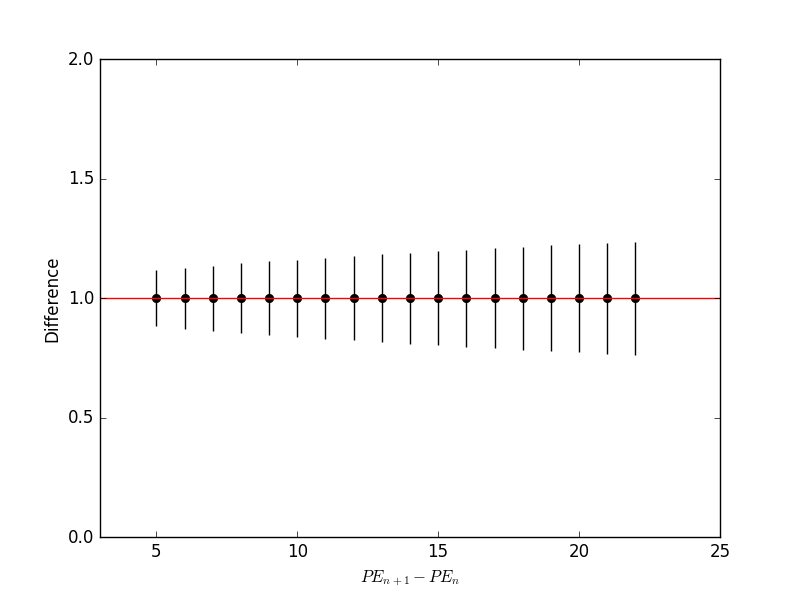
\includegraphics[scale=0.45]{imm/pos.png}
\end{center}
\caption{\mytokens{position_diff} results for gaussian spectrum.}
\label{fig:12}
\end{figure}
A non-linearity result it could be caused by a wrong \verb|tollerance| value or a possible signal saturation.
\newpage
\subsection{Fit of integrated area}
\label{par:area}
After making sure that \mytokens{fwhm_lin} and \mytokens{position_diff} have accorded results to SiPM physics, the integrated spectrum should be right for analysis and physical interpretation.\\
Integrated final area is the result of integrated single n-PE areas. I wrote a script called \mytokens{fit_area} that makes the following operation:
\begin{equation}
Area_n = A_n\cdot \sigma_n \cdot \sqrt{2\pi}
\end{equation}
where $A_n$ is the n-peak amplitude. In the same script there is a fit function too that can choose to linear or gaussian fit for the final spectrum. I tested this script on the simulated gaussian spectrum showed in fig~\ref{fig:6}. The result in fig~\ref{fig:13}.

\begin{figure}[!h]
\begin{center}
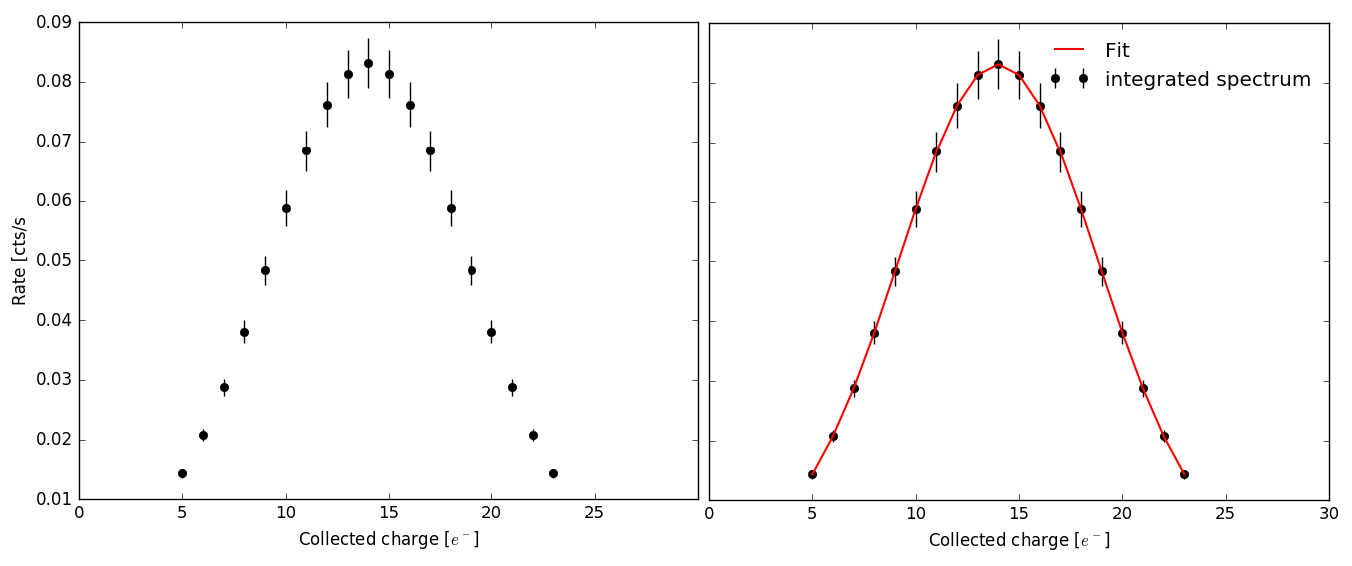
\includegraphics[scale=0.33]{imm/area_fit.png}
\end{center}
\caption{\mytokens{fit_area} results for gaussian spectrum.}
\label{fig:13}
\end{figure}
\newpage

The gaussian result could be a photo-peak detection (as in my case) and the fit results give us information as peak position , resolution and counts per second.\\
The final step of testing software is to compare the integrated spectrum with the original gaussian showed in fig~\ref{fig:4}. Compared values are reported in fig~\ref{fig:14} that makes 1-$\sigma$ accordance between simulation and integration.
\begin{figure}[!h]
\begin{center}
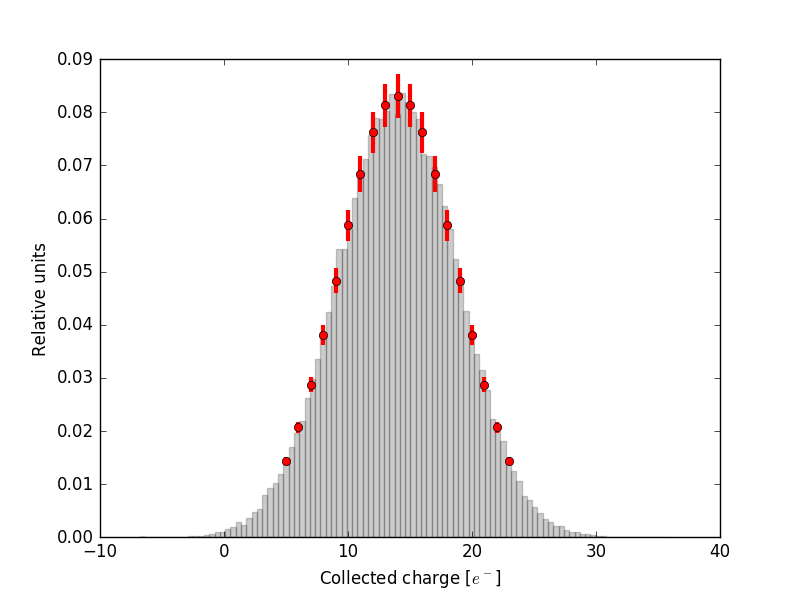
\includegraphics[scale=0.5]{imm/g3.png}
\end{center}
\caption{Comparison between simulated and SiPM post-processed spectrum}
\label{fig:14}
\end{figure}
\end{document}